\documentclass[12pt, openany, oneside]{book}

\usepackage{listings}
\usepackage[dvipsnames]{xcolor}
\usepackage{ctex}
\usepackage{fontspec}
\usepackage{setspace}
\usepackage{tikz}
\usepackage{anyfontsize}
\usepackage{sectsty}
\usepackage{titlesec}
\usepackage{float}
\usepackage[hidelinks]{hyperref}
\usepackage[a4paper]{geometry}
\usepackage{url}
\usepackage{amssymb}
\usepackage{fontawesome5}
\usepackage[most]{tcolorbox}
\usepackage{stackengine}
\usepackage{multirow}
\usepackage{makecell}
\usepackage[T1]{fontenc}
\usepackage{diagbox}
\usepackage{longtable}
\usepackage{newtxtt}
\usepackage{pgf-umlcd}
\usepackage{bbding}
\usepackage{amsmath}
\usepackage{tkz-graph}
\usepackage{drawstack}
\usepackage{dcolumn}
\usepackage{tikzpeople}

\usetikzlibrary{calc,positioning,arrows,fit,shapes}
\usetikzlibrary{shapes.multipart,chains}
\usetikzlibrary{shadows}
\usetikzlibrary{arrows.meta}
\usetikzlibrary{matrix,backgrounds}
\usetikzlibrary{automata}

\tikzset{block/.style={
        font=\sffamily,
        draw=black,
        thin,
        fill=pink!50,
        rectangle split,
        rectangle split horizontal,
        rectangle split parts=#1,
        outer sep=0pt},
        gblock/.style={
            block,
            rectangle split parts=#1,
            fill=green!30}
        }

\makeatletter
\newcommand{\verbatimfont}[1]{\renewcommand{\verbatim@font}{\ttfamily#1}}
\makeatother

\makeatletter
\def\BState{\State\hskip-\ALG@thistlm}
\makeatother

\def\rlwd{.5pt} \def\rlht{2.2ex} \def\rldp{.5ex}
\def\mydiv#1{~
  \rule[-\rldp]{\rlwd}{\rlht}
  \setbox0=\hbox{~#1}
  \stackunder[\dimexpr\rldp-\rlwd]{~#1}{\rule{\wd0}{\rlwd}}
}

\definecolor{mycolor}{RGB}{0,128,128}
\newtcbox{\mybox} {
    on line,
    colback=mycolor,
    fontupper=\bfseries\color{white},
    boxrule=0pt,
    arc=5pt, 
    boxsep=0pt, 
    left=2pt, 
    right=2pt, 
    top=5pt, 
    bottom=5pt
}

\setstretch{1.5}
\setlength{\parindent}{0cm}

\geometry{a4paper,top=2.5cm,bottom=2.5cm}

\titleformat{\chapter}{\Huge\Huge\bfseries}{\chaptertitlename\ \thechapter{\ }}{0pt}{\Huge}{}
\titlespacing{\chapter}{0pt}{0pt}{12pt}

\definecolor{dkgreen}{rgb}{0,0.4,0}
\definecolor{gray}{rgb}{0.5,0.5,0.5}
\definecolor{mauve}{rgb}{0.58,0,0.82}
\definecolor{LightGray}{gray}{0.9}

\lstset{
    basicstyle=\linespread{1.3} \fontspec{Consolas},    %  the size of the fonts that are used for the code
	basewidth=0.5em,
    numbers=left,            % where to put the line-numbers
    numberstyle=\color{black},  % the style that is used for the line-numbers
    numbersep=10pt,                  % how far the line-numbers are from the code
    backgroundcolor=\color{white},
    showspaces=false,
    showstringspaces=false,
    showtabs=false,
    frame=single,                   % adds a frame around the code
    rulecolor=\color{black},        % if not set, the frame-color may be changed on line-breaks within not-black text (e.g. commens (green here))
    tabsize=4,                      % sets default tabsize to 2 spaces
    captionpos=t,                   % sets the caption-position to bottom
    breaklines=false,                % sets automatic line breaking
    breakatwhitespace=true,        % sets if automatic breaks should only happen at whitespace
    title=\lstname,                   % show the filename of files included with \lstinputlisting;
    % also try caption instead of title
    numberstyle=\color{black},		% line number color
    keywordstyle=\color{blue},          % keyword style
    commentstyle=\color{dkgreen},       % comment style
    stringstyle=\color{mauve},         % string literal style
    escapeinside={\%*}{*)},            % if you want to add LaTeX within your code
    morekeywords={*,...}               % if you want to add more keywords to the set
}

\begin{document}

\thispagestyle{empty}

\begin{tikzpicture}[overlay,remember picture]
	\fill[
		black!2]
	(current page.south west) rectangle (current page.north east);

	\shade[
		left color=Dandelion,
		right color=Dandelion!40,
		transform canvas ={rotate around ={45:($(current page.north west)+(0,-6)$)}}]
	($(current page.north west)+(0,-6)$) rectangle ++(9,1.5);

	\shade[
		left color=lightgray,
		right color=lightgray!50,
		rounded corners=0.75cm,
		transform canvas ={rotate around ={45:($(current page.north west)+(.5,-10)$)}}]
	($(current page.north west)+(0.5,-10)$) rectangle ++(15,1.5);

	\shade[
		left color=lightgray,
		rounded corners=0.3cm,
		transform canvas ={rotate around ={45:($(current page.north west)+(.5,-10)$)}}] ($(current page.north west)+(1.5,-9.55)$) rectangle ++(7,.6);

	\shade[
		left color=orange!80,
		right color=orange!60,
		rounded corners=0.4cm,
		transform canvas ={rotate around ={45:($(current page.north)+(-1.5,-3)$)}}]
	($(current page.north)+(-1.5,-3)$) rectangle ++(9,0.8);

	\shade[
		left color=red!80,
		right color=red!80,
		rounded corners=0.9cm,
		transform canvas ={rotate around ={45:($(current page.north)+(-3,-8)$)}}] ($(current page.north)+(-3,-8)$) rectangle ++(15,1.8);

	\shade[
		left color=orange,
		right color=Dandelion,
		rounded corners=0.9cm,
		transform canvas ={rotate around ={45:($(current page.north west)+(4,-15.5)$)}}]
	($(current page.north west)+(4,-15.5)$) rectangle ++(30,1.8);

	\shade[
		left color=RoyalBlue,
		right color=Emerald,
		rounded corners=0.75cm,
		transform canvas ={rotate around ={45:($(current page.north west)+(13,-10)$)}}]
	($(current page.north west)+(13,-10)$) rectangle ++(15,1.5);

	\shade[
		left color=lightgray,
		rounded corners=0.3cm,
		transform canvas ={rotate around ={45:($(current page.north west)+(18,-8)$)}}]
	($(current page.north west)+(18,-8)$) rectangle ++(15,0.6);

	\shade[
		left color=lightgray,
		rounded corners=0.4cm,
		transform canvas ={rotate around ={45:($(current page.north west)+(19,-5.65)$)}}]
	($(current page.north west)+(19,-5.65)$) rectangle ++(15,0.8);

	\shade[
		left color=OrangeRed,
		right color=red!80,
		rounded corners=0.6cm,
		transform canvas ={rotate around ={45:($(current page.north west)+(20,-9)$)}}]
	($(current page.north west)+(20,-9)$) rectangle ++(14,1.2);

	% Title
	\node[align=center] at ($(current page.center)+(0,-7)$)
	{
	{\fontsize{60}{60} \selectfont {{软件工程}}}\\[1cm]
	{\fontsize{40}{40} \selectfont {{Software Engineering}}}\\[2cm]
	{\fontsize{20}{19.2} \selectfont \textcolor{orange}{ \bf 极夜酱}}\\[4pt]
	};
\end{tikzpicture}

\newpage

\pagestyle{plain}
\setcounter{page}{1}
\setcounter{tocdepth}{1}
\tableofcontents

\newpage

\setcounter{page}{1}

% \chapter{需求工程}

\section{软件开发}

\subsection{软件开发}

什么是好的软件?一个好的软件需要满足三点要求:

\begin{enumerate}
    \item 一般要求(general requirements)
    \item 法律要求(legal requirements)
    \item 具体要求(specific requirements)
\end{enumerate}

一般要求包括软件系统需要有详细的文档、可读性高的代码、易于修改和维护的代码、能够开展测试、容易移植、使用方便等方面。\\

法律要求表示系统必须要遵守相关的法律法规。例如加拿大安大略省制定了残疾人无障碍法案,要求软件必须考虑照顾到残障人士的使用;加拿大反垃圾邮件立法规制了垃圾邮件、间谍软件、恶意软件和僵尸网络等问题。\\

具体要求即来自客户和用户具体的需求,软件系统应该要能够实现客户和用户提出的功能。\\

想要开发出一款好的软件,必须要拥有良好的编程能力,这可以通过大量练习提高。同时也需要具备良好的沟通和规划能力,例如在处理问题时,应该与客户或者熟悉问题的人沟通,确保理解了客户/用户的需求。编程前也可以先查找别人已经做过的相关内容,不要重复造轮子。

\newpage

\section{需求}

\subsection{用户故事(User Story)}

用户故事是用几句话描述用户会做的一件事,以及他们为什么要这样做。用户故事是关于用户将会做什么,而不是怎么做。\\

用户故事一般采用这样的格式:“As a [user type], I want [some action] so that [some reason].”。例如,“作为一个活跃用户,我想不用每次登录都输入账号密码,以便更方便快速地登录。”\\

\subsection{需求(Requirements)}

需求描述了软件做的某一件事,它可以是功能性(functional)或非功能性(non-functional)的。同样一个需求只需要描述做什么,而不是如何去做。\\

需求的作用是为了让开发者和客户都清楚最终产品想要的预期是什么。\\

一个好的需求应该具备以下条件:

\begin{itemize}
    \item 分类(categorized):使用MuSCOW法则对需求进行分类。
          \begin{itemize}
              \item MUSTS:系统能够满足客户的基本需求,类似于最小可行产品(minimum viable product)
              \item SHOULDS:满足客户基本或更高级的需求
              \item COULDS:能够使系统变得更好的额外需求
              \item WON'TS:系统不该做的事情
          \end{itemize}

    \item 有优先级(prioritized):对不同的需求指定一个优先级,需要遵守MUSTS > SHOULDS > COULDS > WONT'S。

    \item 逻辑合理:需求之间的依赖关系需要合理,例如一个MUST需求不能依赖于一个SHOULD需求。

    \item 时间估计(time estimate):一个需求应该需要在15天内完成,如果不能完成, 应该把它分解成多个小需求。
\end{itemize}

\newpage

\section{原型设计}

\subsection{原型设计(Prototyping)}

原型是指没有功能的模型,它不一定要包含一个程序的所有方面。\\

原型设计是与客户/用户沟通的一种工具,让客户/用户感觉他们自己也是设计者。原型设计的目的是为了验证UI是否能够可以被正常使用,让开发者能够以用户的角度思考问题。\\

\subsection{纸上原型(Paper Prototyping)}

纸上原型也称低保真原型(low fidelity prototyping),通过纸笔等工具设计,通常是UI设计的第一步。它具有制作过程快速、成本低、更改快速、效率高的特点。\\

\begin{figure}[H]
    \centering
    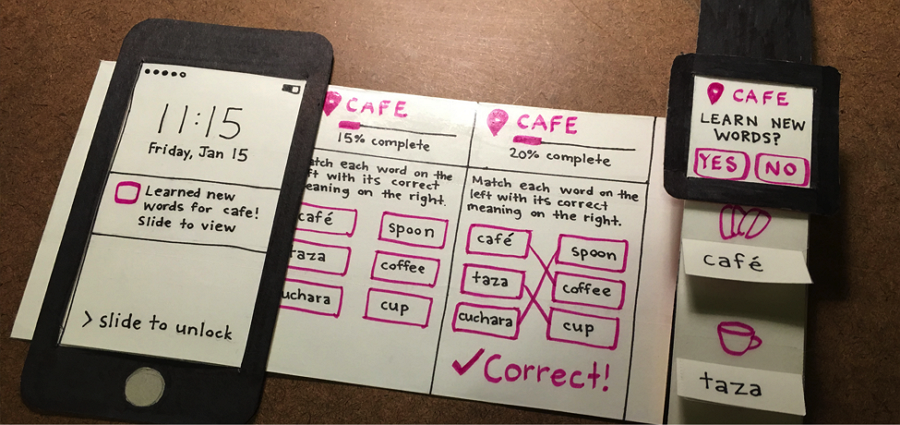
\includegraphics[scale=0.5]{img/C1/1-3/1.png}
    \caption{纸上原型}
\end{figure}

\begin{figure}[H]
    \centering
    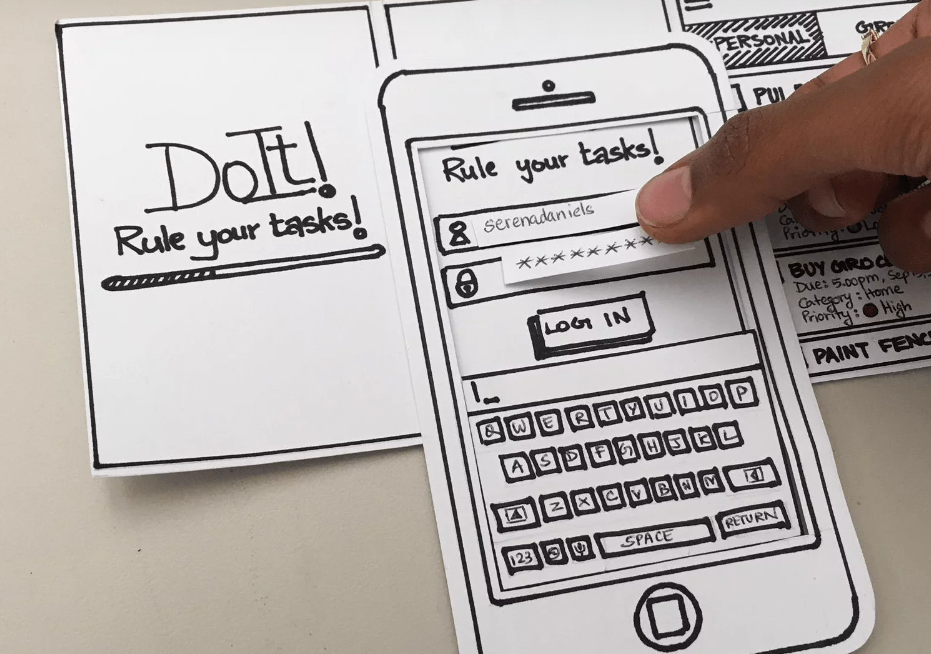
\includegraphics[scale=0.7]{img/C1/1-3/2.png}
    \caption{纸上原型}
\end{figure}

纸上原型的目的并不是为了让UI更加美观,而是为了确保系统的流程是否存在问题。\\

在完成纸上原型后,需要让参与测试的人根据用例进行测试。在测试过程中,不要提供任何帮助或者指导,以此来验证用户交互是否流畅。\\

最后,记录下在纸上原型测试中哪些地方是正常的、哪些地方存在问题或遗漏的。\\

\subsection{线框图(Wireframing)}

线框图也称高保真原型(high fidelity prototyping),它看上去非常接近最终产品,几乎完全按照实物来制作,原型中甚至包含产品的细节、真实的交互、UI等。\\

\begin{figure}[H]
    \centering
    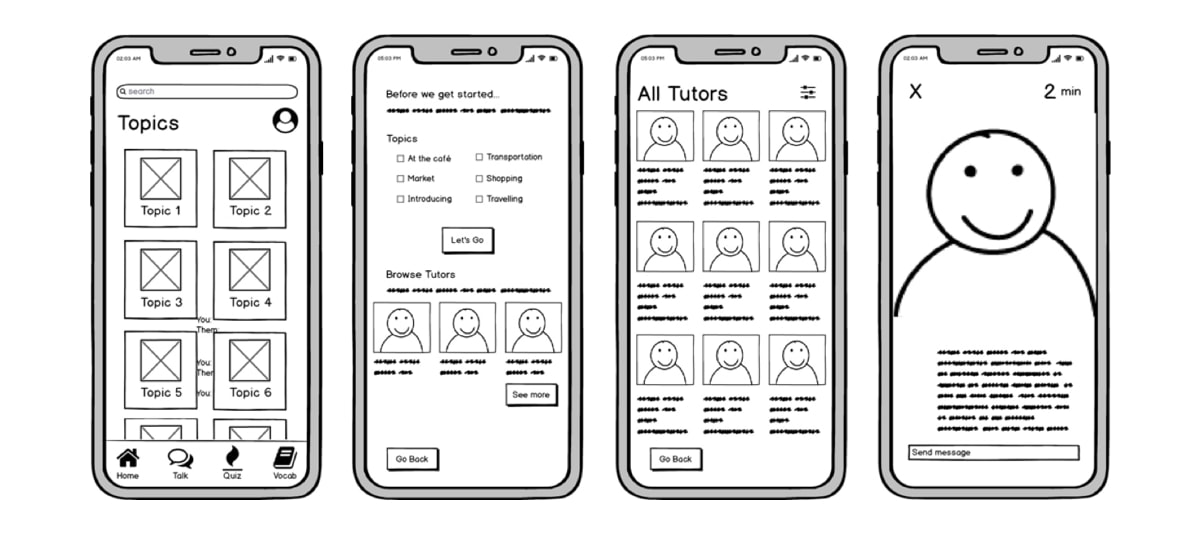
\includegraphics[scale=0.35]{img/C1/1-3/3.png}
    \caption{线框图}
\end{figure}

\begin{figure}[H]
    \centering
    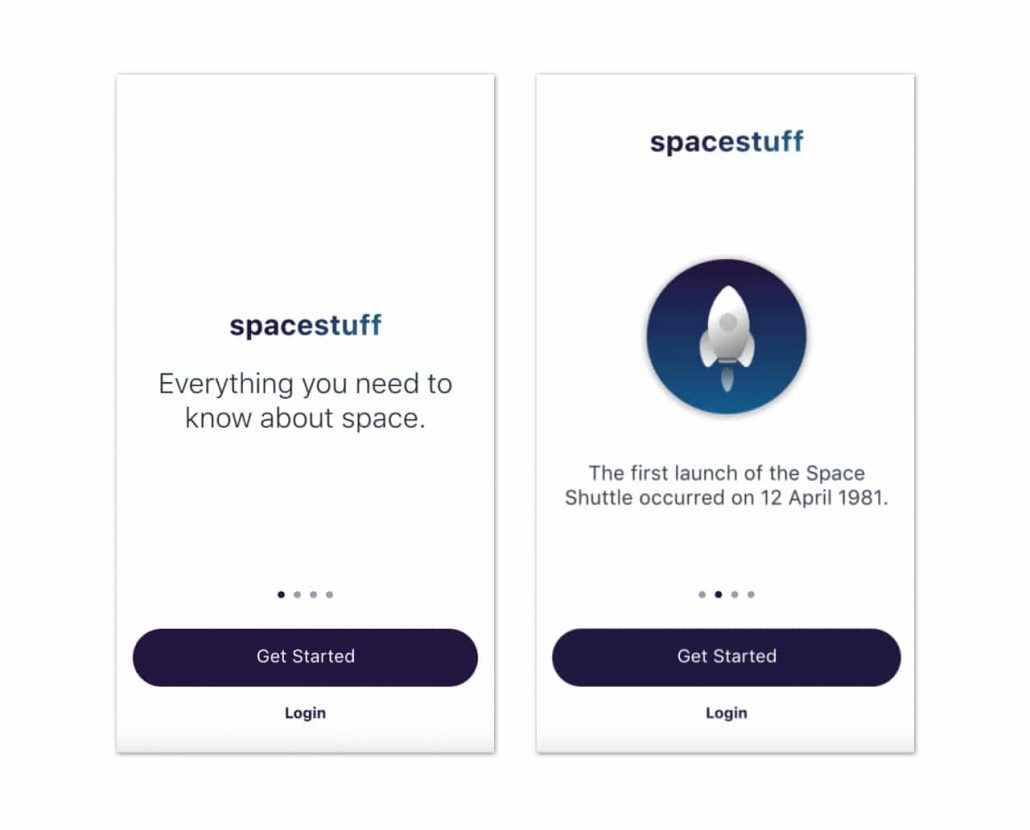
\includegraphics[scale=0.5]{img/C1/1-3/4.png}
    \caption{线框图}
\end{figure}

高保真原型的目的在于让用户提供反馈,例如UI中控件的位置和UI的美观程度。

\newpage

\end{document}